\documentclass{report}
\newcommand{\projectName}{SAP}
\usepackage[bookmarks=true]{hyperref}
\usepackage[dvipsnames]{xcolor}
\usepackage{graphicx} % Required for inserting images
\usepackage{tcolorbox}
\usepackage{multicol}
\usepackage{xcolor}
\usepackage{subfigure}
\usepackage{wrapfig}

\usepackage[pages=some]{background}

\definecolor{lightgreen}{RGB}{237, 239, 234}
\definecolor{lightblue}{RGB}{234, 237, 239}
\definecolor{lightred}{RGB}{239, 234, 237}

\RequirePackage{graphicx, pdfpages, pdflscape, pgfplots, tcolorbox, graphbox}

%
\usepackage[utf8]{inputenc}
\usepackage{titlesec}
\usepackage{eso-pic}
\usepackage[framemethod=tikz]{mdframed}
\usepackage[square,numbers]{natbib}
\AtBeginDocument{
  \renewcommand{\bibsection}{\chapter{\bibname}}
} % Bibliography in numbered chapter

\usepackage{geometry}
\usepackage{amsmath}
\usepackage{parskip}
\usepackage[official]{eurosym}
\setlength {\marginparwidth}{2cm} 
\usepackage{todonotes}
\usepackage{csquotes}

\usepackage{rotating}
\usepackage{lmodern}
\usepackage{setspace}


\hypersetup{
    %bookmarks=false,    % show bookmarks bar?
    pdftitle={Software Requirement Specification},    % title
    pdfauthor={Bharat-Krishn-Prathyush-Sujeeth},                     % author
    pdfsubject={\projectName Software Requirements Specification},                        % subject of the document
    pdfkeywords={SRS, client, use cases}, % list of keywords
    colorlinks=true,       % false: boxed links; true: colored links
    linkcolor=Dandelion,       % color of internal links
    citecolor=Bittersweet,      % color of links to bibliography
    filecolor=Periwinkle,        % color of file links
    urlcolor=PineGreen, % WildStrawberry        % color of external links
    linktoc=page            % only page is linked
}



\title{SWEProjectTeam18CoAP}
\author{Krishn Kher}
\date{\today}

\begin{document}
\setlength{\footskip}{50pt}
\BgThispage
% used packages in the template
% import your package here 


\begin{center}
\vspace*{1cm}

\backgroundsetup{
scale=1,
color=black,
opacity=0.15,
angle=0,
contents={%
  
\includegraphics[width=\paperwidth,height=\paperheight]{images/SRS_Frontpage.png}
  }%
}

\begin{figure}[t]
  \raggedleft 
  \begin{minipage}{1cm}
  
\includegraphics[width=3cm]{images/IITH_Logo.png}
  \end{minipage}
\end{figure}

\vspace*{2cm}

\vspace*{0.1in}
%yellow version
\AddToShipoutPictureBG*{\AtPageLowerLeft{% 
  \color{OliveGreen}\rule{.16 \paperwidth}{\paperheight} }
   \:
   \:
   \;
   \;
   \:
  \begin{turn}{90} 
   \fontsize{35}{80}\selectfont \textbf{\color{SpringGreen} 
 ~\texttt{\projectName~SRS Documentation}}
  \end{turn}
  
  }

\begin{spacing}{1.7}

\begin{tabular}{p{4cm} ll}

& \textbf{\huge \projectName: Seat Allotment Portal}\\ % Here the title of your work \\
& \Large Software Requirements Specification \\ % Here the title of your work
& \\
& \large \textbf{\texttt{Course}}: Software Engineering \\
& \large \textbf{\texttt{Course code}}: \texttt{CS4443} \\

& \\
& \large \textbf{\texttt{Faculty Guide}}: \textit{Dr. MV Panduranga Rao} \\
& \large \textbf{\texttt{Student Developers}}: \\
& \large Bhavanam Sujeeth Kumar Reddy (\texttt{ES19BTECH11022}) \\
& \large Krishn Vishwas Kher (\texttt{CS19B23P000001}) \\
& \large Mukkavalli Bharat Chandra (\texttt{ES19BTECH11015}) \\
& \large Sree Prathyush Chinta (\texttt{CS19BTECH11043}) \\
& \\
& \\
& \begin{tcolorbox}[colframe=white, colback=Apricot, arc=8pt, boxrule=4mm, boxsep=1mm] \textbf{\texttt{Seat Allotment Portal}} tailored for managing CoAP/GATE admisssions @ IITH.
\end{tcolorbox} \\ 
\end{tabular}
\end{spacing}
\end{center}



\thispagestyle{empty} % Prevents page number from being included on the cover
\clearpage\setcounter{page}{1} % Start including page numbers from here
\pagenumbering{arabic} % in roman numerals
\tableofcontents
\clearpage

\chapter{Introduction}
\section{Purpose}
\begin{tcolorbox}[colframe=white, colback=lightblue, arc=8pt] Our system is designed to make it more convenient for the members of the student shortlisting committee dealing with the applications for PG programmes offered at the institute by allocating the seats to the students automatically with 100 \% accuracy.
This document provides an overview of the characteristics of our system, giving the client a lucid picture of the product we offer alongside serving as a roadmap for our developers. \end{tcolorbox}

\section{Scope}
Below enumerated are the aspects of our system that fall within the scope of our system as well as those that fall out of it.
\subsection{In scope}
\begin{tcolorbox}[colframe=white, colback=lightgreen, arc=8pt]
\begin{itemize}
    \item Performing the seat allocation process across various rounds of CoAP procedure.
    \item Sorting the users based on priorities as well as raising exception errors when ties occur for various candidates.
    \item Modification of seat matrix at any point during the CoAP process.
    \item Providing statistics of seat allotment after the entire CoAP process.
    \item User authentication.
\end{itemize}
\end{tcolorbox}
\subsection{Out of scope}
\begin{tcolorbox}[colframe=white, colback=lightred, arc=8pt]
\begin{itemize}
    \item Uploading the seat allotment output to the CoAP portal.
    \item Downloading the CoAP response from the portal.
    \item Verification of user details before sorting.
\end{itemize}
\end{tcolorbox}
\section{Definitions, Acronyms, and Abbreviations}
Documentation of computerese and associated meanings that will be used frequently in this document and in subsequent software documents for this project.
\subsection{Abbreviations \& Acronyms}
\begin{itemize}
    \item \textbf{\textcolor{magenta}{SAP}}: Seat Allotment Portal.
    \item \textbf{\textcolor{magenta}{CoAP}}: Common Offer Acceptance Portal.
    \item \textbf{\textcolor{magenta}{PG}}: Post Graduate.
\end{itemize}
\subsection{Definitions}
\begin{itemize}
    \item \textbf{Sorting}: Ordering the candidates based on the priorities specified by the user.
    \item \textbf{Seat Matrix}: The seats count division across various specialisations and subsequent divisions based on category (under each specialisation), as mandated by the user.
\end{itemize}
\section{References}
\begin{enumerate}
    \item \textbf{Appendix A}: Sorting procedure used by the portal. (\ref{Appendix A})
    \item \textbf{Appendix B}: Seat Matrix declaration and modification. (\ref{Appendix B})
    \item \textbf{Appendix C}: User Interface. (\ref{Appendix C})
\end{enumerate}
\newpage
\section{Overview}
\begin{itemize}
    \item \textbf{Section $2$}: Provides a comprehensive overview of the software, including the expected level of proficiency for users, general constraints that must be considered during software development, as well as the underlying assumptions and dependencies. 
    \item \textbf{Section $3$}: We will delve into the specific requirements that the software must fulfill, with functional requirements presented through various use cases. Additionally, performance requirements and design constraints will also be detailed in this section.
    \item \textbf{Section $4$}: Here we will shed light on potential future extensions for the system, which will be of great interest to those who plan to use the software in the long term.
    \item \textbf{Section $5$}: Describes few crucial processes that can occur during the seat allocation procedure.  
\end{itemize}
\chapter{Overall description}
\section{Product Perspective}
\begin{tcolorbox}[colframe=white, colback=lightblue, arc=8pt]
    The “Seat Allotment Portal” software is aimed for IITH faculty to sort the candidates based on a sorting criteria efficiently and to reduce the manual component involved with the traditional method significantly. 
    SAP should be an easy-to-use, highly reliable software capable of offering a lot of flexibility to the user(s). SAP is intended to be a stand-alone software, independent of the availability of other software. 
    SAP is platform independent, i.e, it should run on Linux, UNIX and Windows based platforms. 
\end{tcolorbox}
\newpage
\section{Product Functions}
\begin{figure}[h!]
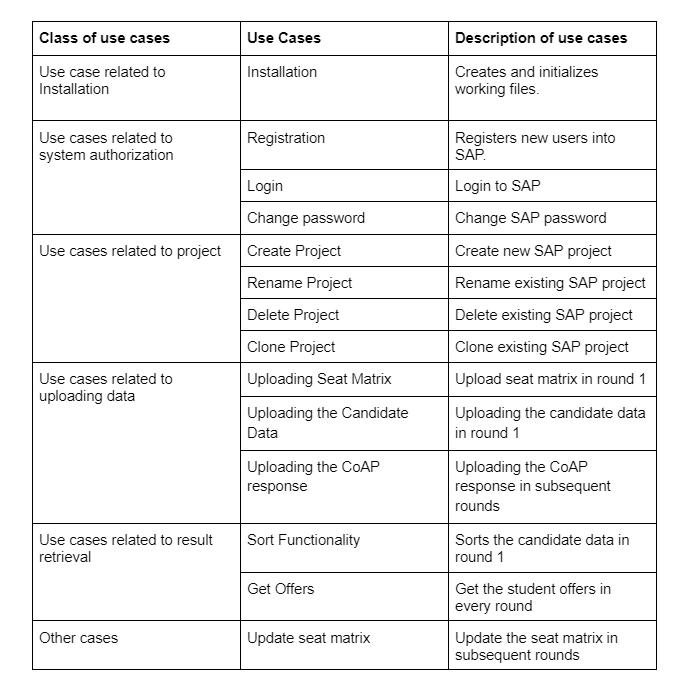
\includegraphics[width=\textwidth]{images/table.png}
\end{figure}
\section{Product Planning}
Agile methodology will be adopted to ensure the maximum client satisfaction as well as continuous delivery of working code after every few sprints. Code practices that facilitate continuous feedback from the users will be always strived for. This may include changing certain details in the present SRS document, but the barebone structure will remain invariant.
\section{User Characteristics}
\begin{itemize}
    \item The intended user is a person empowered by IITH with the academic powers authorized to shortlist students based on various criteria e.g. faculty member of IITH.
    \item The user should be familiar with the rules needed for shortlisting. 
    \item Familiarly with basic handling of Microsoft Excel/Google sheets is desirable.
\end{itemize}
\section{Principal Actors}
    \begin{itemize}
        \item \texttt{\textbf{\textcolor{TealBlue}{User}}}.
        \item \texttt{\textbf{\textcolor{TealBlue}{System}}}.
    \end{itemize}
\section{General Constraints}
\begin{enumerate}
    \item Should output results with 100\% accuracy.
    \item It should be efficiently scalable in the number of students being shortlisted.
    \item Tool/application should be OS-independent.
    \item Requires Internet connection for it to work fully.
\end{enumerate}
\section{Assumptions \& Dependencies}
\begin{enumerate}
    \item Certain features require Internet connectivity.
    \item Takes input data only in the form of Microsoft Excel /Google sheets/csv files.
    \item $100$\% accuracy on results guaranteed only when data is $100$\% clean.
    \item The user uploads the correct .csv file containing the candidates data in Round $1$.
\end{enumerate}

\chapter{Specific Requirements}
\section{Functional Requirements}
The functional requirements are described via various use cases.
\subsection{Installation}
\begin{tcolorbox}[colframe=white, colback=lightblue, arc=8pt]
\begin{itemize}
    \item \textbf{Use Case $1$} \textit{Installation of SAP}\\
    \begin{itemize}
        \item \textbf{Primary Actor}: User.
        \item \textbf{Precondition}: Internet connection available.
        \item \textbf{Main scenario}: \begin{enumerate}
            \item The user installs the SAP tool from the IITH intranet. 
            \item System asks the user for the home directory in which all the working files will be created.
        \end{enumerate}
       \item \textbf{Alternate Scenario}: 
       \begin{enumerate}
           \item Network failure - Installation aborted.
       \end{enumerate}
    \end{itemize}
\end{itemize}
\end{tcolorbox}
\subsection{System Authorization}
\begin{tcolorbox}[colframe=white, colback=lightred, arc=8pt]
\begin{itemize}
    \item \textbf{Use Case $2$} \textit{Registration on SAP
}\\
    \begin{itemize}
        \item \textbf{Primary Actor}: User.
        \item \textbf{Precondition}: User must have installed SAP.
        \item \textbf{Main scenario}: \begin{enumerate}
            \item User gives the IITH email address.
            \item User enters the desired password. 
            \item User re-enters the password. 
        \end{enumerate}
       \item \textbf{Alternate Scenario}: 
       \begin{enumerate}
           \item User tries to register multiple times using the same IITH email address yet the user fails to do so. A message saying “Account already exists!” is generated.
       \end{enumerate}
    \end{itemize}
\end{itemize}
\begin{itemize}
    \item \textbf{Use Case $3$} \textit{Login
}\\
    \begin{itemize}
        \item \textbf{Primary Actor}: User.
        \item \textbf{Precondition}: User must have registered on SAP
.
        \item \textbf{Main scenario}: \begin{enumerate}
            \item Start the application. User prompted for login and password. 
            \item User gives the login and password.
            \item System does authentication.
            \item Home page is displayed. 
        \end{enumerate}
       \item \textbf{Alternate Scenario}: 
       \begin{enumerate}
           \item 
           \begin{itemize} 
           \item Authorization fails.
            \item Prompt the user that he typed the wrong password.
            \item Allow him to re-enter the password.
           \end{itemize}
           \item 
           \begin{itemize}
           \item  User logins through multiple devices.
           \item Log out from the current session.
           \item Warns the user to login only through a single device.
           \end{itemize}
       \end{enumerate}
    \end{itemize}
\end{itemize}

\begin{itemize}
    \item \textbf{Use Case $4$} \textit{Change Password
}\\
    \begin{itemize}
        \item \textbf{Primary Actor}: User.
        \item \textbf{Precondition}: User logged in.
        \item \textbf{Main scenario}: \begin{enumerate}
            \item User goes to the profile settings page to change the password. 
            \item User is prompted for old password, new password and confirm new password.
            \item User gives the old password, new password and confirms the new password.
            \item System does authentication.
            \item New password is registered with the system.
        \end{enumerate}
       \item \textbf{Alternate Scenario}: 
       \begin{enumerate}
           \item 
           \begin{itemize} 
           \item Authorization fails.
            \item Prompt the user that he typed the wrong password.
            \item Allow him to re-enter the password.
           \end{itemize}
           \item 
           \begin{itemize}
           \item New password and the confirmed new password do not match.
           \item Allow him to re-enter the attributes. 
           \end{itemize}
       \end{enumerate}
    \end{itemize}
\end{itemize}
\end{tcolorbox}

\subsection{Project}
\begin{tcolorbox}[colframe=white, colback=lightgreen, arc=8pt]
\begin{itemize}
    \item \textbf{Use Case $5$} \textit{Create Project
}\\
    \begin{itemize}
        \item \textbf{Primary Actor}: User.
        \item \textbf{Precondition}: User logged in.
        \item \textbf{Main scenario}: \begin{enumerate}
            \item User initiates the “Create Project” functionality. 
            \item System asks the user for the project name.
            \item User enters the project name.
            \item An empty project is created.
        \end{enumerate}
       \item \textbf{Alternate Scenario}: 
       \begin{enumerate}
           \item 
           \begin{itemize} 
           \item Project with the same name exists.
            \item System asks the user for a different name.
            \item User enters a different name.
            \item Empty project gets created.
           \end{itemize}
       \end{enumerate}
    \end{itemize}
\end{itemize}   

\begin{itemize}
    \item \textbf{Use Case $6$} \textit{Rename Project
}\\
    \begin{itemize}
        \item \textbf{Primary Actor}: User.
        \item \textbf{Precondition}: User should have an existing project
        \item \textbf{Main scenario}: \begin{enumerate}
            \item User initiates the “rename project” functionality. 
            \item System asks for the project to be renamed and the new name.
            \item User enters the new name.
            \item Project is renamed.
        \end{enumerate}
       \item \textbf{Alternate Scenario}: 
       \begin{enumerate}
           \item 
           \begin{itemize} 
           \item Project with the same name exists.
            \item System asks the user for a different name.
            \item User enters a different name.
            \item Project gets renamed.
           \end{itemize}
       \end{enumerate}
    \end{itemize}
\end{itemize}

\begin{itemize}
    \item \textbf{Use Case $7$} \textit{Delete Project
}\\
    \begin{itemize}
        \item \textbf{Primary Actor}: User.
        \item \textbf{Precondition}: User should have an existing project
        \item \textbf{Main scenario}: \begin{enumerate}
            \item User selects a project. 
            \item User selects the “Delete Project” functionality for the selected project.
            \item The system deletes the project.
        \end{enumerate}
       \item \textbf{Alternate Scenario}: 
       \begin{enumerate}
           \item 
           None
       \end{enumerate}
    \end{itemize}
\end{itemize}
\end{tcolorbox}

\begin{tcolorbox}[colframe=white, colback=lightgreen, arc=8pt]
\begin{itemize}
    \item \textbf{Use Case $8$} \textit{Clone Project
}\\
    \begin{itemize}
        \item \textbf{Primary Actor}: User.
        \item \textbf{Precondition}: User should have an existing project
        \item \textbf{Main scenario}: \begin{enumerate}
            \item User selects a project. 
            \item User selects the “Clone Project” functionality for the selected project.
            \item System creates a duplicate project with a system generated name.
        \end{enumerate}
       \item \textbf{Alternate Scenario}: 
       \begin{enumerate}
           \item 
           None
       \end{enumerate}
    \end{itemize}
\end{itemize}
\end{tcolorbox}

\subsection{Data uploads}
\begin{tcolorbox}[colframe=white, colback=lightblue, arc=8pt]

\begin{itemize}
    \item \textbf{Use Case $9$} \textit{Uploading Seat Matrix
}\\
    \begin{itemize}
        \item \textbf{Primary Actor}: User.
        \item \textbf{Precondition}: User has created a new project and has selected Round 1.
        \item \textbf{Main scenario}: \begin{enumerate}
            \item User either uploads the csv file containing the seat matrix or manually fills in the seat matrix in SAP. 
            \item The seat matrix has been successfully uploaded to SAP.
        \end{enumerate}
       \item \textbf{Alternate Scenario}: 
       \begin{enumerate}
           \item 
           \begin{itemize} 
           \item If a user violates the seat matrix format in SAP in the uploaded csv file.
            \item System generates a warning message.
            \item The user is prompted to upload the file again.
           \end{itemize}
       \end{enumerate}
    \end{itemize}
\end{itemize}   

\begin{itemize}
    \item \textbf{Use Case $10$} \textit{Uploading the Candidate Data in Round 1
}\\
    \begin{itemize}
        \item \textbf{Primary Actor}: User.
        \item \textbf{Precondition}: User has uploaded the seat matrix
        \item \textbf{Main scenario}: \begin{enumerate}
            \item User uploads the candidate data (csv file) on SAP. 
            \item The upload is successful.
            \item Preview of the uploaded csv file is shown on the screen.
        \end{enumerate}
       \item \textbf{Alternate Scenario}: 
       \begin{enumerate}
           \item 
           None
       \end{enumerate}
    \end{itemize}
\end{itemize}   
\end{tcolorbox}
\begin{tcolorbox}[colframe=white, colback=lightblue, arc=8pt]

\begin{itemize}
    \item \textbf{Use Case $11$} \textit{Upload the CoAP response
}\\
    \begin{itemize}
        \item \textbf{Primary Actor}: User.
        \item \textbf{Precondition}: User is accessing a subsequent round (not Round 1)
        \item \textbf{Main scenario}: \begin{enumerate}
            \item User uploads the CoAP response of the previous round and generates a new list of offers for that particular round. 
        \end{enumerate}
       \item \textbf{Alternate Scenario}: 
       \begin{enumerate}
           \item 
           \begin{itemize}
               \item User should upload the correct CoAP response file. A prompt will be generated if an incorrect file is uploaded.
           \end{itemize}
       \end{enumerate}
    \end{itemize}
\end{itemize}
    
\end{tcolorbox}

\subsection{Result retrieval}
\begin{tcolorbox}[colframe=white, colback=lightred, arc=8pt]

\begin{itemize}
    \item \textbf{Use Case $12$} \textit{Sort Candidate Data
}\\
    \begin{itemize}
        \item \textbf{Primary Actor}: User.
        \item \textbf{Precondition}: User has uploaded the candidate data in Round 1.
        \item \textbf{Main scenario}: \begin{enumerate}
            \item User sets the sorting criteria by selecting the columns (from the existing columns in the candidate data) based on a priority criteria. 
            \item The user selects either ascending or descending order for each priority.
            \item The user saves the sorting preferences.
            \item User initializes the “Sort Candidate Data” functionality.
            \item System sorts the candidate data according to the user sorting criteria.
        \end{enumerate}
       \item \textbf{Alternate Scenario}: 
       \begin{enumerate}
           \item 
           \begin{itemize} 
           \item After sorting the file, if there are multiple ties, the user is prompted to give additional rules to break the ties to proceed with the following steps.
           \end{itemize}
       \end{enumerate}
    \end{itemize}
\end{itemize}

\begin{itemize}
    \item \textbf{Use Case $13$} \textit{Get Offers
}\\
    \begin{itemize}
        \item \textbf{Primary Actor}: User.
        \item \textbf{Precondition}: Use has sorted the candidate data.
        \item \textbf{Main scenario}: \begin{enumerate}
            \item User initializes the “Get Offers” functionality to download the offers made to the students in the particular round. 
            \item The downloaded csv file will be in a format required by the CoAP portal.
        \end{enumerate}
       \item \textbf{Alternate Scenario}: 
       \begin{enumerate}
           \item 
           None
       \end{enumerate}
    \end{itemize}
\end{itemize}
    
\end{tcolorbox}


\subsection{Others}
\begin{tcolorbox}[colframe=white, colback=lightgreen, arc=8pt]

\begin{itemize}
    \item \textbf{Use Case $14$} \textit{Update seat matrix in subsequent rounds (except Round 1)
}\\
    \begin{itemize}
        \item \textbf{Primary Actor}: User.
        \item \textbf{Precondition}: Seat matrix has changed in between the CoAP rounds.
        \item \textbf{Main scenario}: \begin{enumerate}
            \item The user changes the seat matrix in between the CoAP rounds. 
        \end{enumerate}
       \item \textbf{Alternate Scenario}: 
       \begin{enumerate}
           \item 
           \begin{itemize}
               \item The user cannot decrease the seats in the seat matrix between the CoAP rounds. An attempt to do so will generate a prompt warning the user.
           \end{itemize}
       \end{enumerate}
    \end{itemize}
\end{itemize}

\end{tcolorbox}

\section{Performance Requirements}
\begin{enumerate}
    \item Should be able to run reasonably well even on a low-end laptop.
    \item Should be able to handle large XL files of data, of the order of $1000$s of rows and approximately $100$ columns.
    \item Should run in reasonable time, e.g. roughly an hour for about $2000$ rows and $70$ columns of student data.
\end{enumerate}
\section{Design Constraints}
\begin{itemize}
    \item \textbf{\textit{Security}}: \begin{enumerate}
        \item The user information (username and password) should be encrypted and stored in the server. 
        \item The data that would be uploaded to SAP should be protected from being accessed by external applications that are already present in the user system. 
    \end{enumerate}
    \item \textbf{\textit{Scalability}}: \begin{enumerate}
        \item SAP should be able to handle large .csv files without crashing. 
        \item The SAP server should be able to serve a large number of users simultaneously ($\approx 1000$ users).
    \end{enumerate}
    \item \textbf{\textit{Fault tolerance}}: \begin{enumerate}
        \item Data should not become corrupted in case of a system crash or a power failure.
    \end{enumerate}
    \item \textbf{\textit{Integrity}}: \begin{enumerate}
        \item The input data should be clean.
    \end{enumerate}
\end{itemize}
\section{External Interface Requirements}\label{EIR}
\begin{enumerate}
    \item The application opens with a login window.
    \item Once the user has logged in securely, a window is opened with a sidebar that has the option to create new projects or manage existing ones.
    \item In each project, $10$ rounds can be accessed. A particular round can only be accessed once the previous round is done.
    \item In Round $1$, two csv files must be uploaded to get that round offers, namely the seat matrix csv and candidate data csv. Once the candidate data csv is uploaded, there is a window to preview the csv data. A sort button is also present, which sorts the data based on entered priorities.
    \item Once the sort button is clicked, there is a pop-up that is generated that has the option to add priorities for sorting, for example which column has what priority and even the order to sort in (such as ascending or descending). Then these priorities are saved.
    \item The sorted candidate data can be previewed in the window again. Once this is done, we can download the offers in the format required by CoAP.
    \item In the subsequent rounds, the updated seat matrix and CoAP response .csv files should be uploaded to download that round’s offer.
\end{enumerate}
\chapter{Future Extensions}
\begin{tcolorbox}[colframe=white, colback=lightgreen, arc=8pt]
\begin{enumerate}
    \item Tool should be able to show various statistics about how many offers are in the accept-and-freeze mode/reject-and-wait, etc., which will give the department/institute an idea of the trend across various iterations of the CoAP process. 
    \item Enable the tool to be able to directly send the processed shortlists directly to CoAP.
    \item Handling concurrent transactions across devices for a user.
    \item Tool should support shortlisting based on custom-defined rules that the user can define using a specific protocol rather than just those based on the CoAP shortlisting rule.
\begin{itemize}
    \item Suggest any inconsistencies that might be present in the custom-defined rules.
    \item A further extension would be to enable the user to define the rules in plain English and use NLP to infer the rules being requested for.
\end{itemize}
    \item Enable multilingual data to be input in the data sheets.
    \item Integrate accessibility features into the tool, such as a voice assistant.
    \item Automatic validation of category certificates using state-of-the-art image captioning  techniques.
\end{enumerate}
\end{tcolorbox}
\chapter{Appendix}
\section{Appendix A: Sorting procedure used by the portal}\label{Appendix A}
The sorting procedure used by the portal is flexible and allows the sorting method to be declared by the user, i.e. it allows the user to decide which columns (criteria) should be used to sort the students as well as what ranking to follow with respect to the criteria (selected columns). This allows the user to modify the sorting procedure before the CoAP process starts.
\section{Appendix B: Seat Matrix declaration and modification
}\label{Appendix B}
The seat matrix initial declaration involves either uploading a .csv containing the seat matrix statistics, i.e. the specialization, number of seats, seat type etc., or entering the seat matrix through our portal's input interface.
The seat matrix modification involves changing the statistics of the initially declared statistics i.e. increasing the seats of a specialization. We don't allow for a decrease in the seat count during the modification procedure.
These two procedures together give the user flexibility, which involves accommodating for introduction of new specialization during any given year as well as accommodating seat count changes due to any other action.
\section{Appendix C: User Interface}\label{Appendix C}
The description here comes in a sequel to the External Interface Requirements (\ref{EIR}) described above.
\\

\begin{wrapfigure}{r}{\textwidth}
\fbox{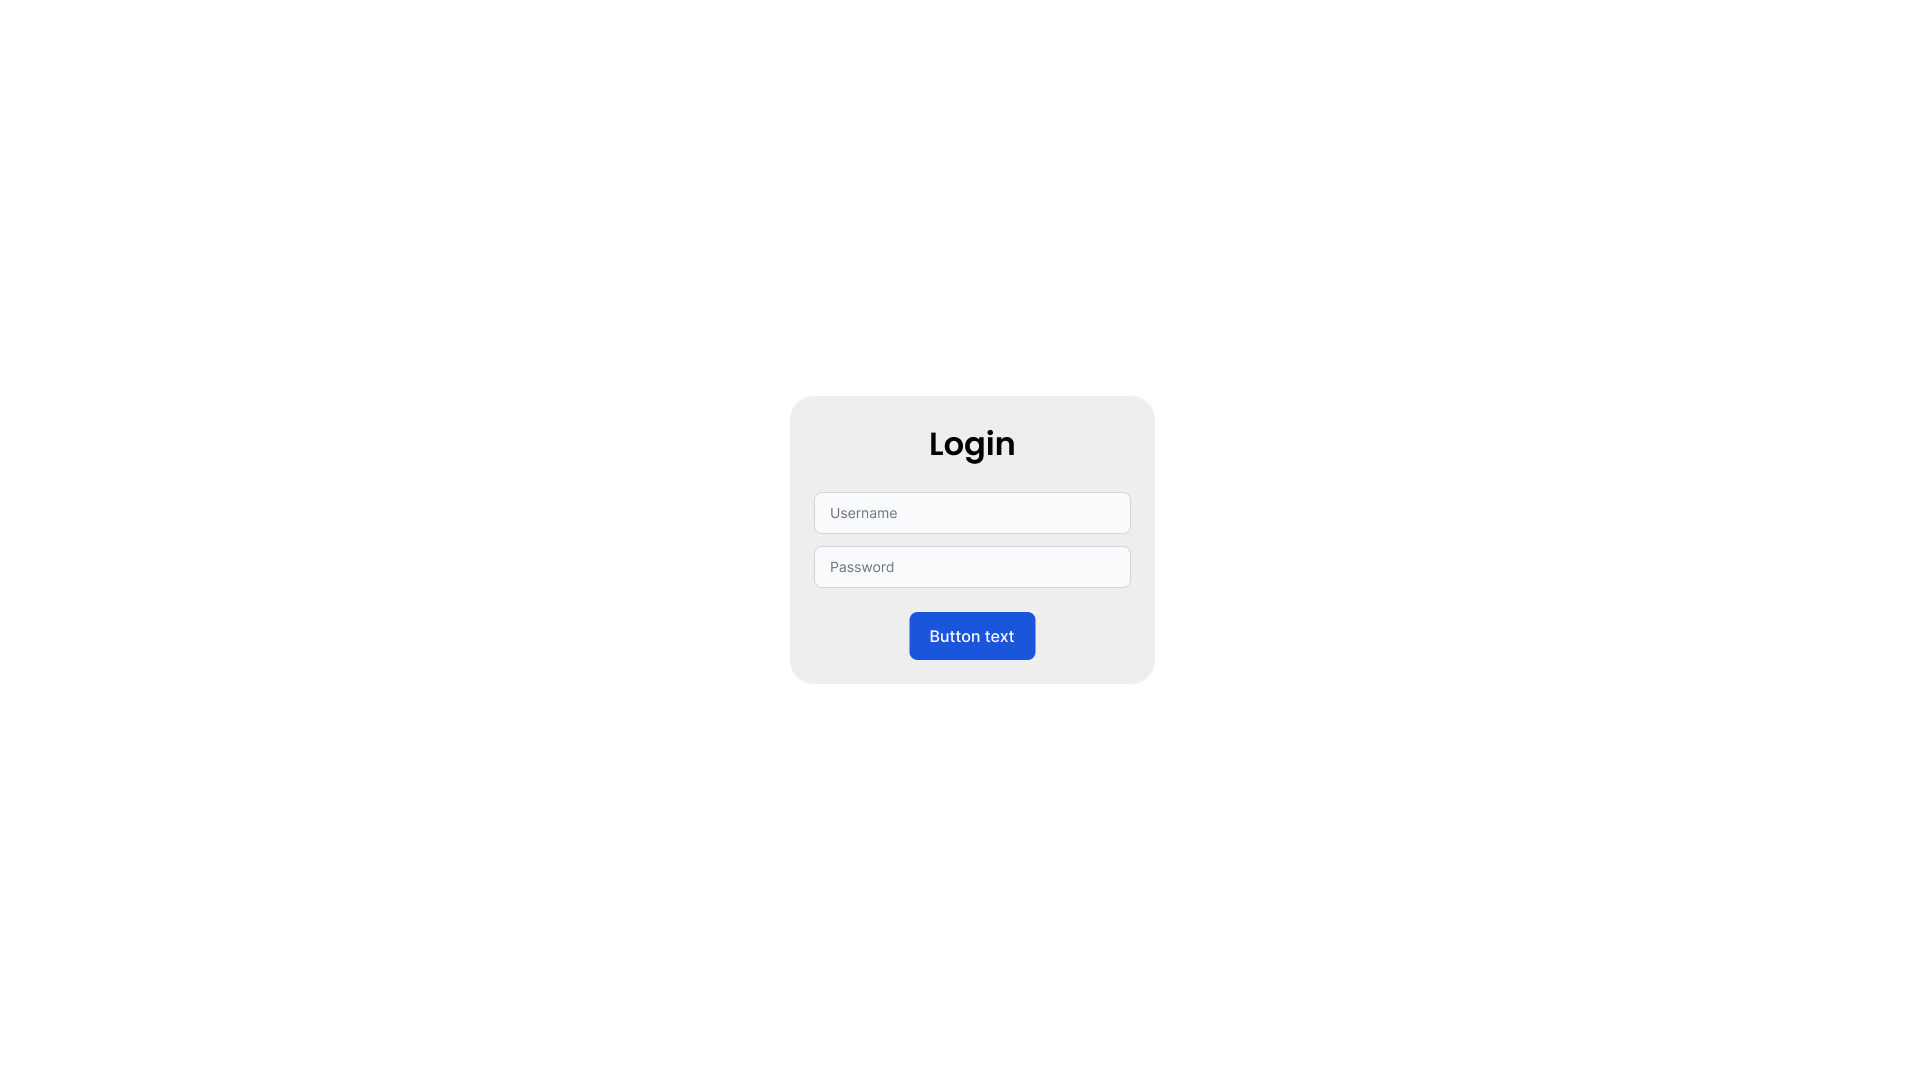
\includegraphics[width=\textwidth]{images/Login.png}}
\caption{The application opens with a login window.}
\end{wrapfigure}

\begin{wrapfigure}{r}{\textwidth}
\fbox{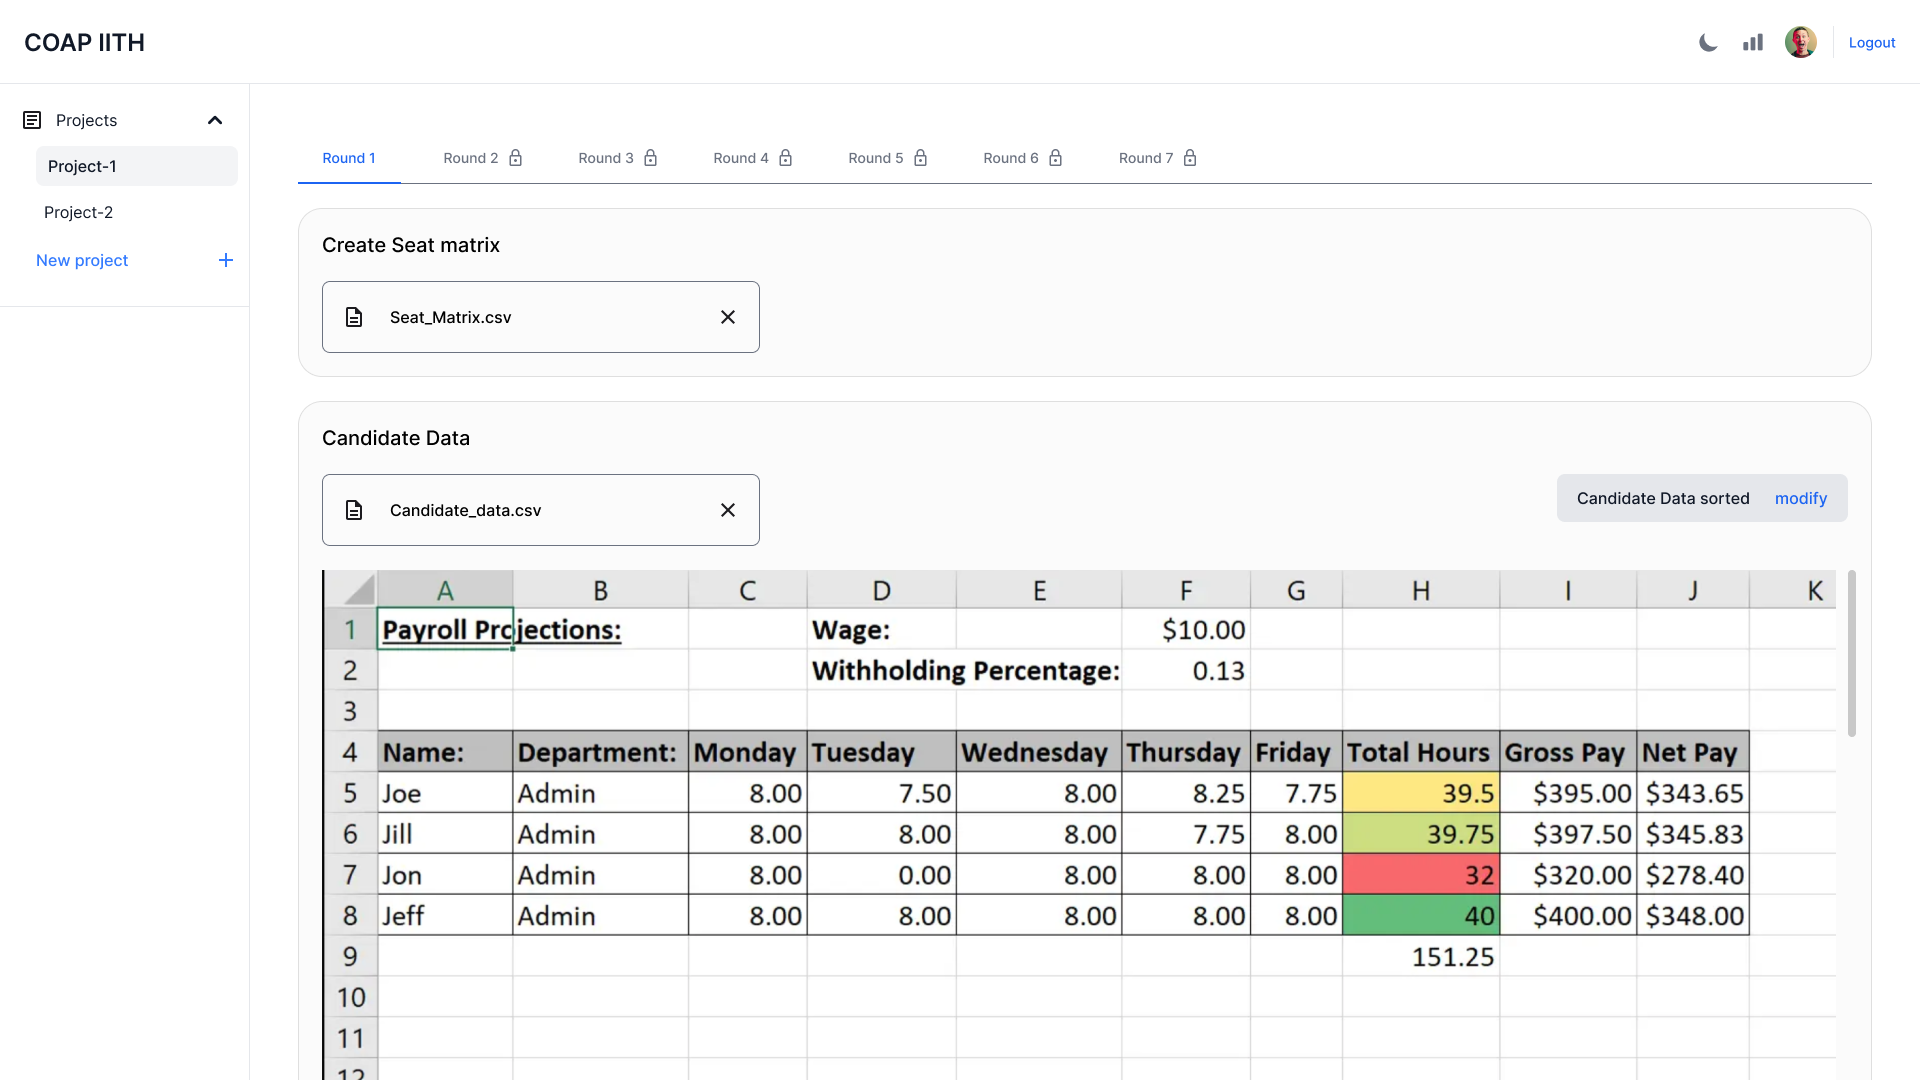
\includegraphics[width=\textwidth]{images/Round 1 - Candidate Data sorted.png}}
\caption{next phase}
\end{wrapfigure}

\begin{wrapfigure}{r}{\textwidth}
\fbox{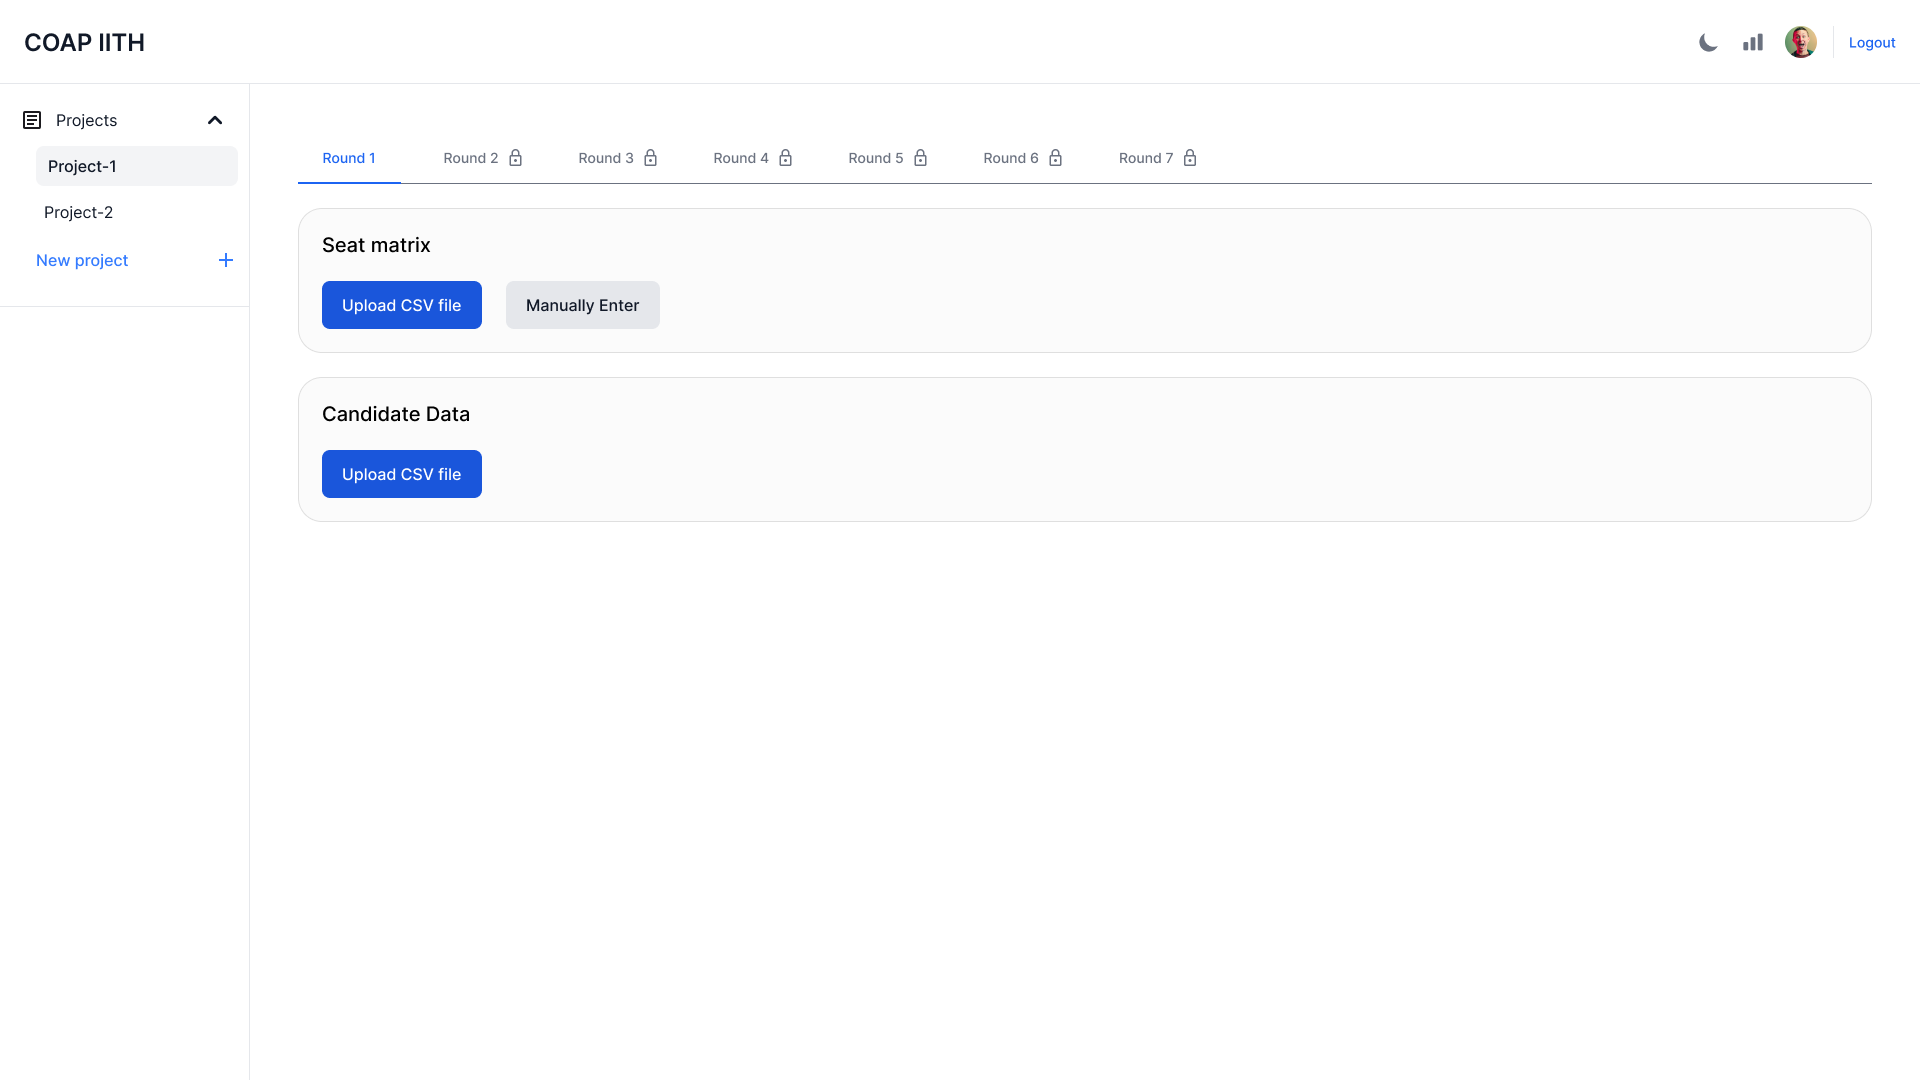
\includegraphics[width=\textwidth]{images/Round 1 - Default.png}}
\caption{Round 1- Default screen.}
\end{wrapfigure}

\begin{wrapfigure}{r}{\textwidth}
\fbox{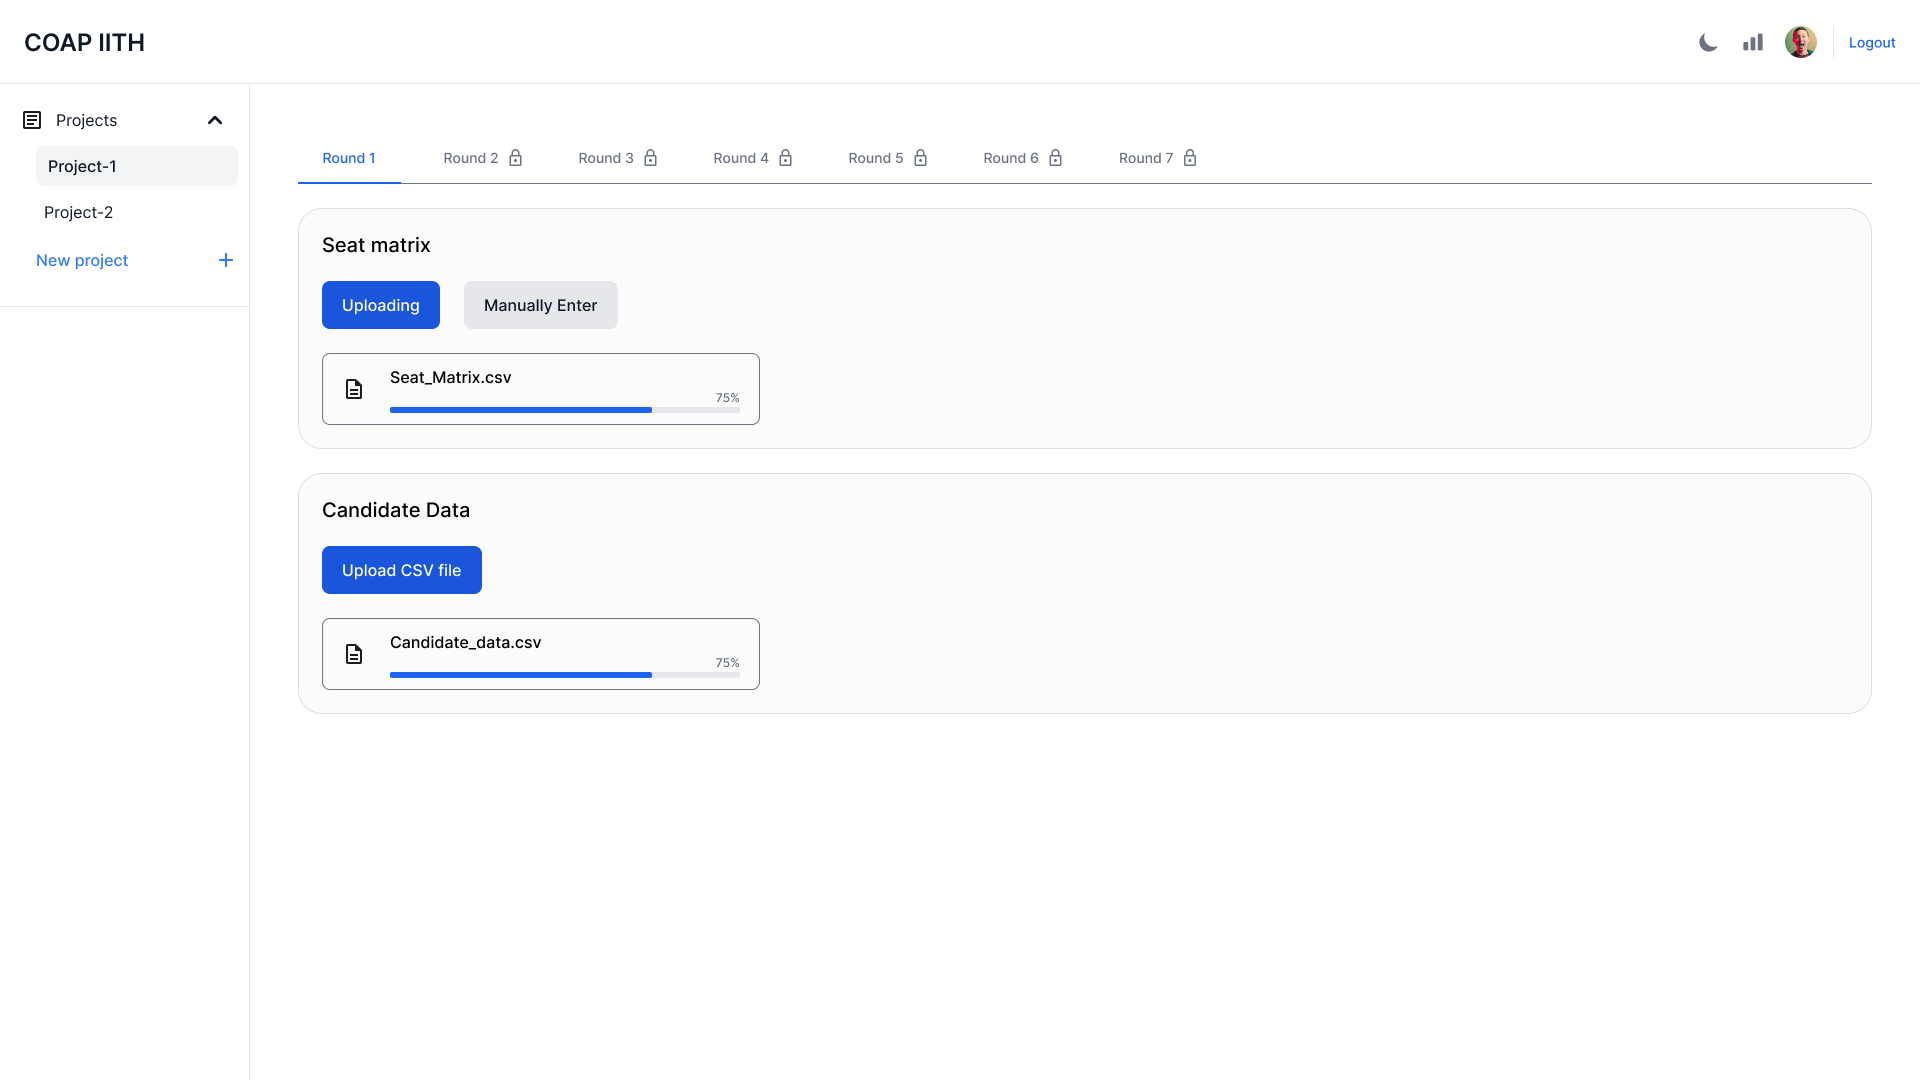
\includegraphics[width=\textwidth]{images/Round 1 - Uploading files.png}}
\caption{Round 1- File Uploading screen.}
\end{wrapfigure}

\begin{wrapfigure}{r}{\textwidth}
\fbox{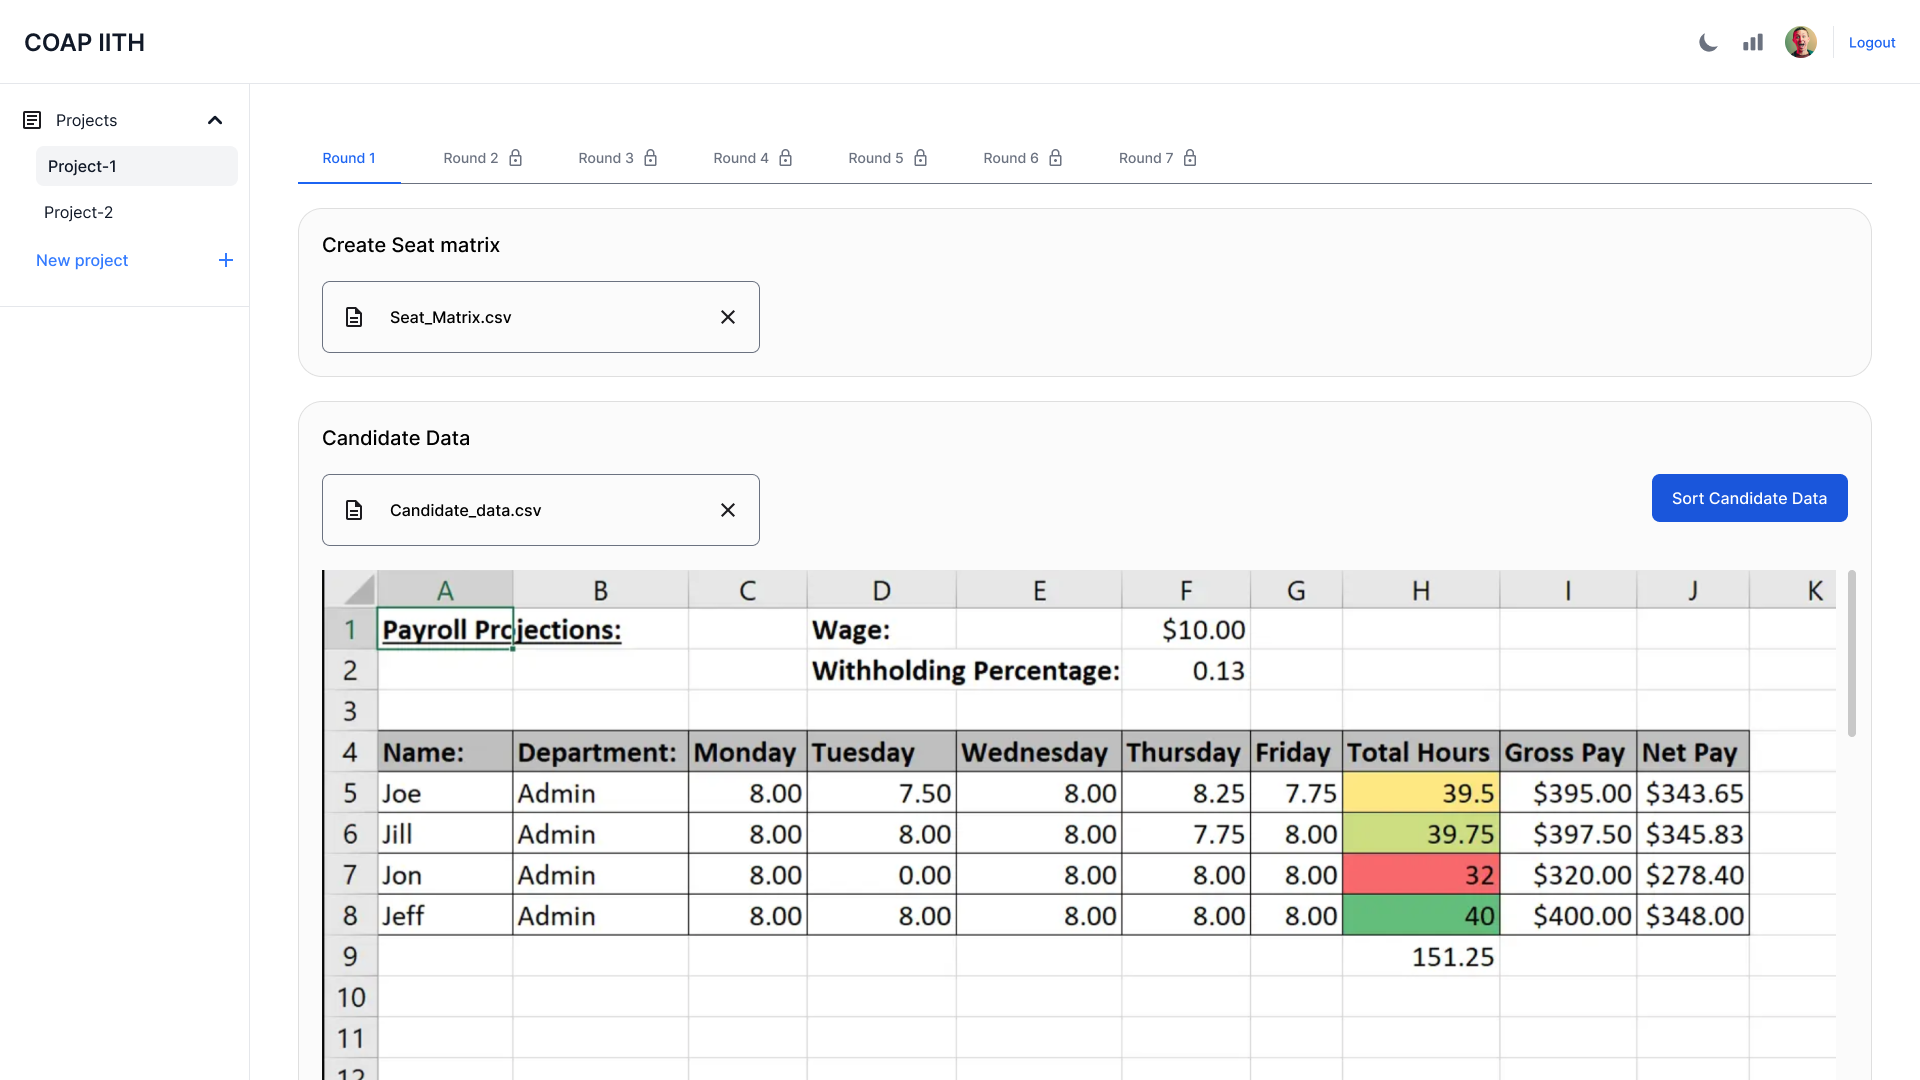
\includegraphics[width=\textwidth]{images/Round 1 - Files Uploaded.png}}
\caption{Round 1- File Uploaded screen.}
\end{wrapfigure}

\begin{wrapfigure}{r}{\textwidth}
\fbox{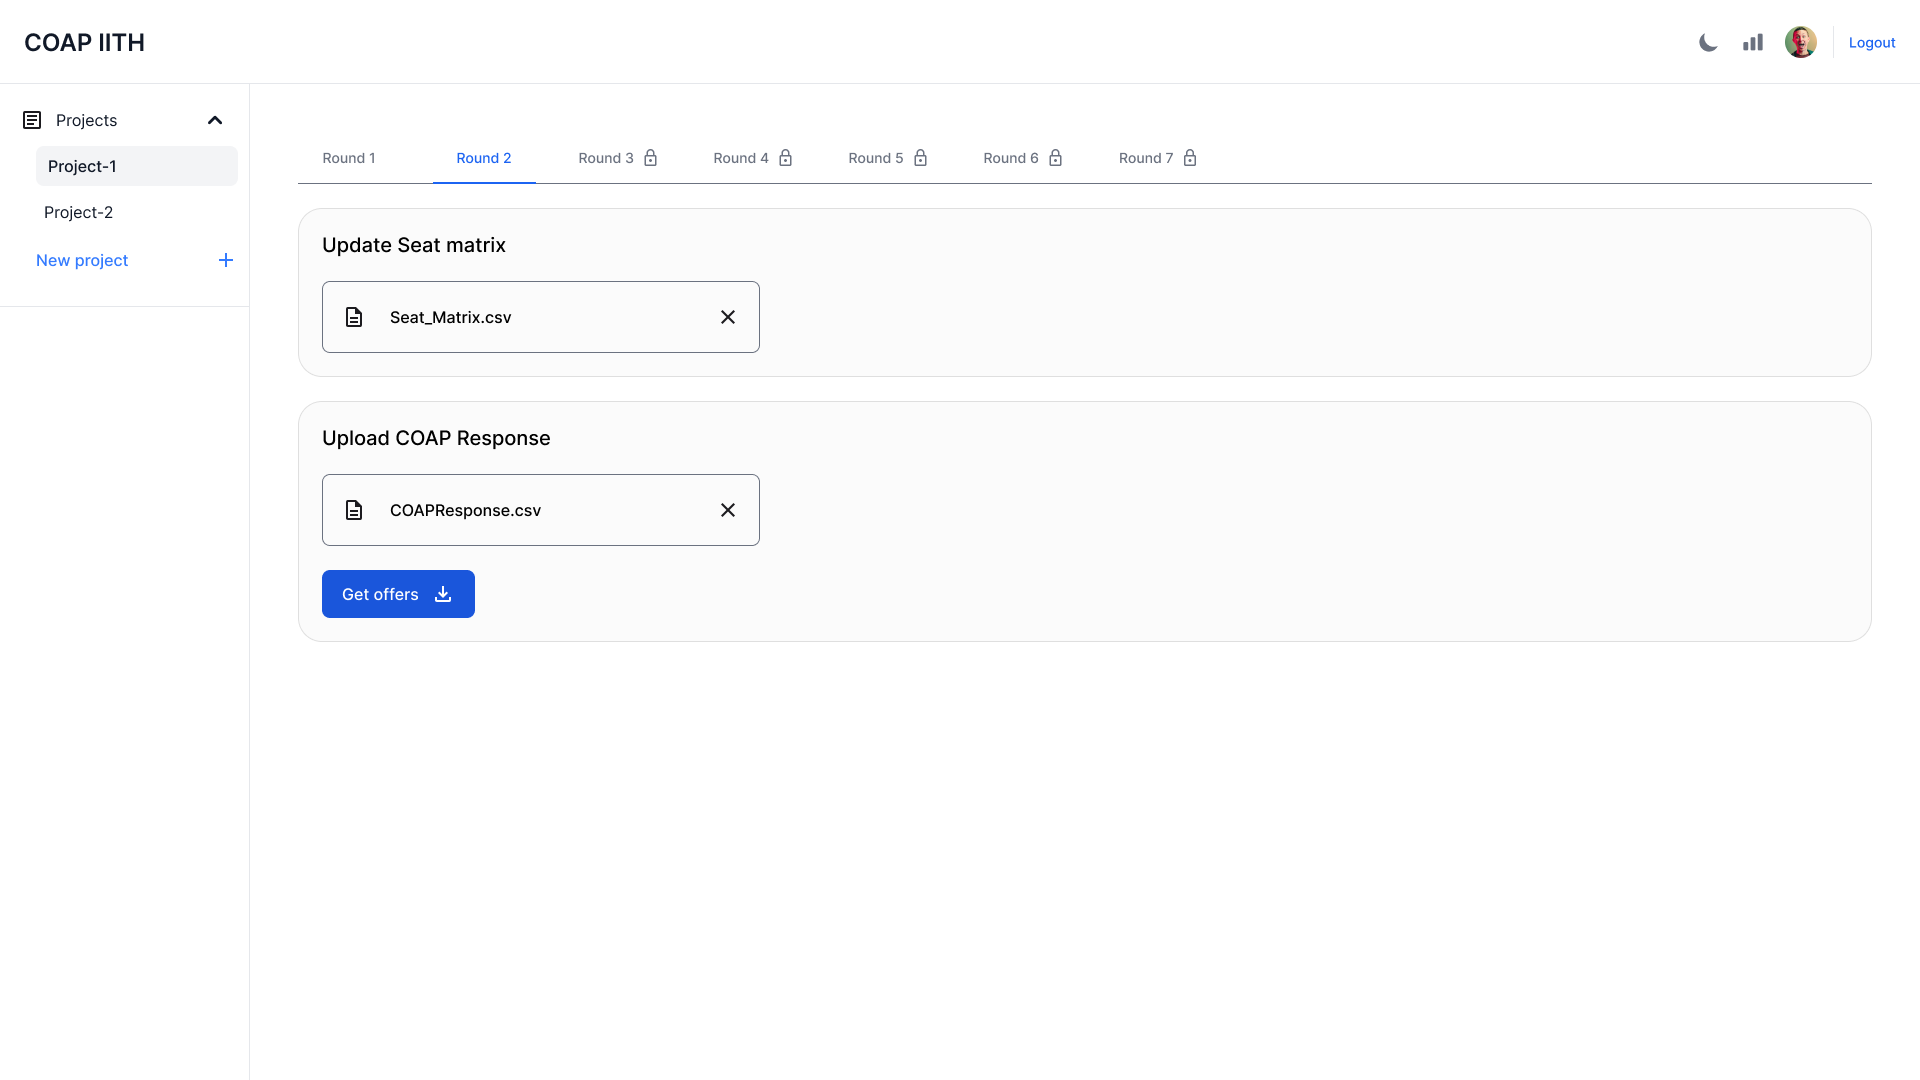
\includegraphics[width=\textwidth]{images/Round 2 - files uploaded.png}}
\caption{Round 2- File Uploaded screen.}
\end{wrapfigure}

\begin{wrapfigure}{r}{\textwidth}
\fbox{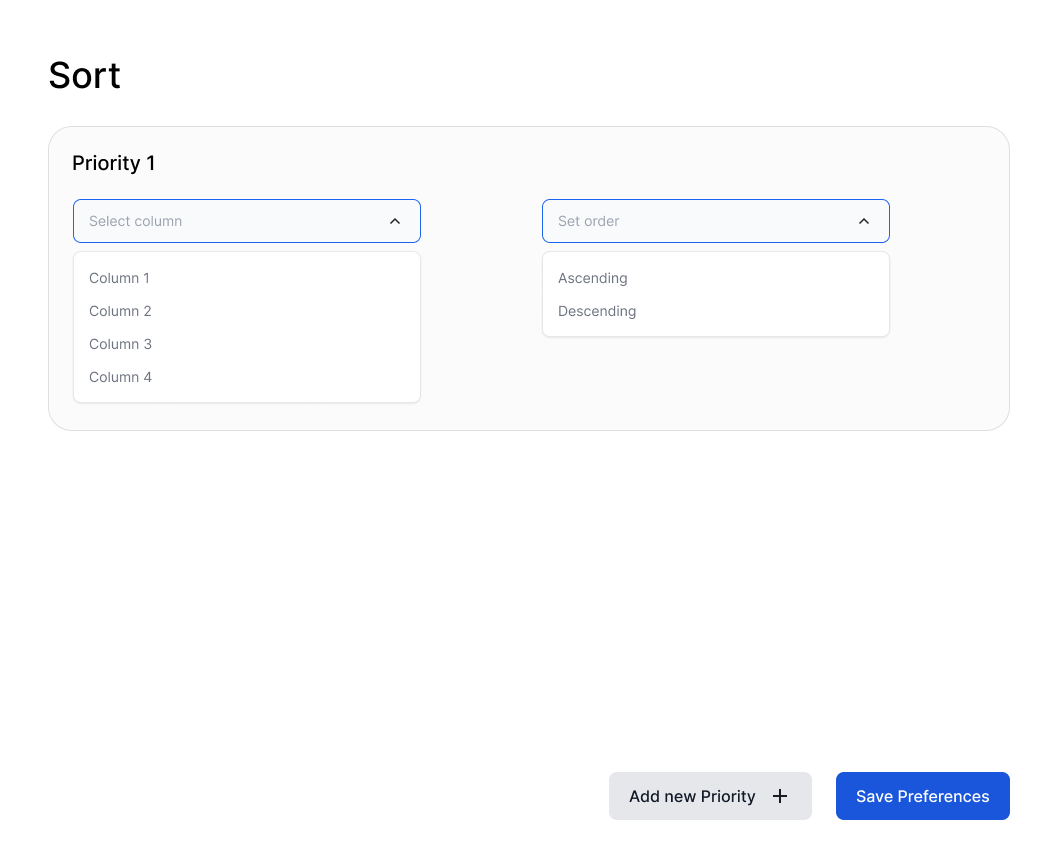
\includegraphics[width=\textwidth]{images/Sort - Dropdown.png}}
\caption{Drop Down for preferences of sorting function.}
\end{wrapfigure}

\begin{wrapfigure}{r}{\textwidth}
\fbox{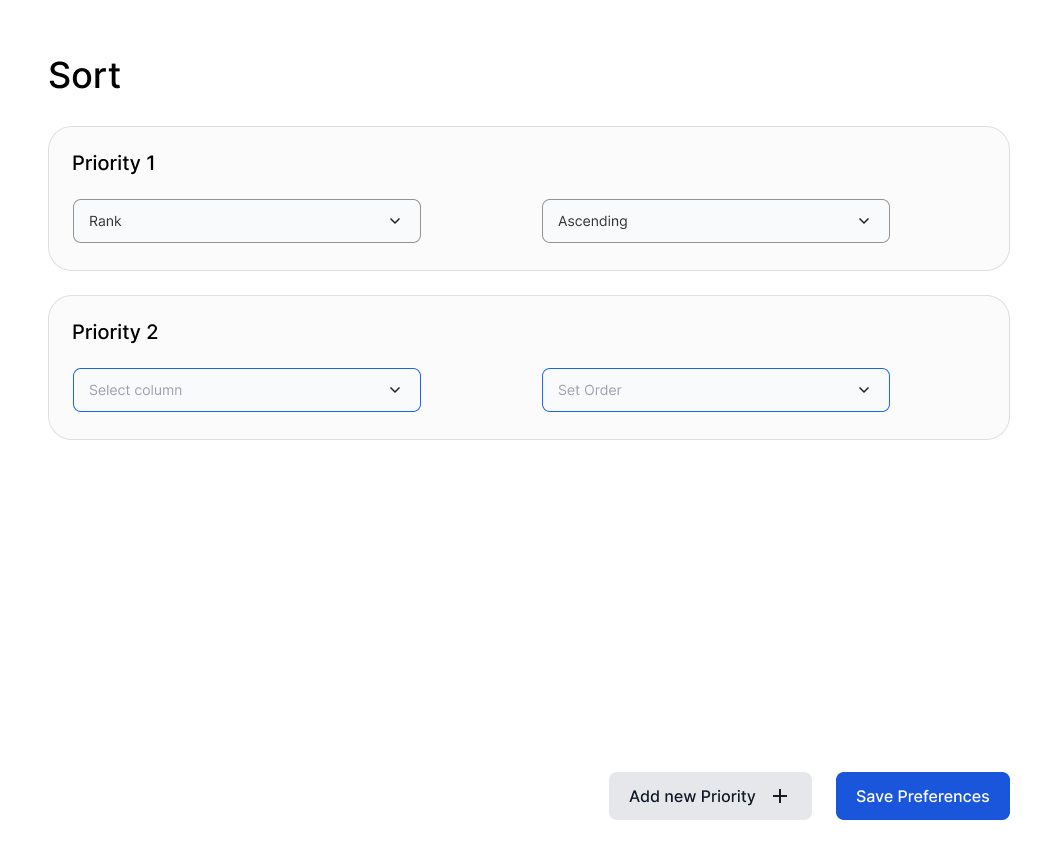
\includegraphics[width=\textwidth]{images/Sort - New preference added.png}}
\caption{New preference added to priority screen for sorting.}
\end{wrapfigure}



\end{document}
